% Solid cut out of the sphere x^2+y^2+z^2=a^2 by the cylinder r = a*cos(theta),
% i.e. (x-a/2)^2 + y^2 = (a/2)^2.  Drawn for a = 1.
% Standalone & compilable with pdflatex (requires the pgfplots package).
\documentclass[tikz,border=3pt]{standalone}
\usepackage{pgfplots}
\pgfplotsset{compat=1.16}

\begin{document}
\begin{tikzpicture}
  \begin{axis}[
      view={35}{22},
      xlabel=$x$, ylabel=$y$, zlabel=$z$,
      width=12cm, height=12cm,
      axis lines=box, clip=false,
      title={sphere $x^{2}+y^{2}+z^{2}=1$ and cylinder $(x-\tfrac12)^{2}+y^{2}=\tfrac14$},
    ]

    % ---- sphere, radius a = 1 ------------------------------------------
    % (theta in [0,360], phi in [0,180])
    \addplot3[
        surf, shader=faceted, opacity=0.18, faceted color=gray!60,
        samples=41, samples y=21,
        domain=0:360, y domain=0:180,
      ]
      ({sin(y)*cos(x)}, {sin(y)*sin(x)}, {cos(y)});

    % ---- cylinder (x-1/2)^2 + y^2 = 1/4 , -1 <= z <= 1 -----------------
    \addplot3[
        surf, shader=faceted, opacity=0.45, color=red!70,
        samples=51, samples y=2,
        domain=0:360, y domain=-1:1,
      ]
      ({0.5+0.5*cos(x)}, {0.5*sin(x)}, {y});

  \end{axis}
\end{tikzpicture}
\end{document}
